\documentclass[12pt,a4paper]{report}
\usepackage[top=1.2in,right=1.2in,left=1.2in,bottom=1in]{geometry}
\usepackage[english,slovene]{babel}
\usepackage[cp1250]{inputenc}
\usepackage[T1]{fontenc}
\usepackage{color}
\usepackage[pdftex]{graphicx}
\usepackage{exscale}
\usepackage{amsmath}
\usepackage{amssymb}
\usepackage[pdftex,bookmarks,colorlinks]{hyperref}
\usepackage{verbatim}
\usepackage[pdftex]{graphicx}
\usepackage{float}		% floating pictures and tables
\usepackage{multirow}	% multirow table input
\usepackage{listings}	% for input of programming code
\usepackage{titlesec}	% for alternative title settings
\usepackage{upgreek}	% for upright greek letters (\upalpha, \upbeta,...)
\usepackage[nomessages]{fp}		% for arithmetics of high precision real point numbers
\usepackage{enumitem}	% for setting spacings in itemize
\usepackage{booktabs}	% nicer tables
\usepackage{epstopdf}	% transforms all eps plots to pdf
\usepackage[titletoc]{appendix}	% for setting appendix chapter title options
\usepackage{url}	% for url links
\usepackage{subfigure} % for making subfigures
\usepackage[]{units}
\usepackage[table]{xcolor}
\usepackage{lineno}
\hypersetup{colorlinks,%
	citecolor=black,%
	filecolor=black,%
	linkcolor=black,%
	urlcolor=blue}

% Packages for nicer computer code
\usepackage{xcolor}
\usepackage{listings}
\lstset{
   basicstyle=\ttfamily\footnotesize,
   columns=fullflexible,
   frame=single,
   breaklines=true,
   postbreak=\mbox{\textcolor{red}{$\hookrightarrow$}\space}
}

% Font type which is much better for reading
\usepackage[sc]{mathpazo}

%\titleformat{\chapter}[hang]{\huge\bf}{\thechapter}{1em}{}
%\titlespacing{\chapter}{0pt}{0pt}{1cm}
\titleformat{\chapter}[hang]{\normalfont\bf}{}{12pt}{\Large\thechapter\enspace}
\titlespacing{\chapter}{0pt}{0pt}{1cm}
\titleformat{\section}[hang]{\normalfont\bf}{}{12pt}{\large\thesection\enspace}
\titleformat{\subsection}[hang]{\normalfont\bf}{}{12pt}{\normalsize\thesubsection\enspace}

% definitions of commands and environments
\newcommand{\diff}{\operatorname{d}\!}	% operator d for integration or differentiation
\newcommand{\pdiff}{\partial}	% operator for partial differentiation
\newcommand{\iu}{{i\mkern1mu}}	% imaginary unit i
\newcommand{\me}{\, \mathrm{e}}	% natural exponential e
\newcommand{\mytilde}{\raise.17ex\hbox{$\scriptstyle\mathtt{\sim}$}}		% tilde sign, denoting similarity
\newcommand{\quotes}[1]{``#1''}	% quotes
\newcommand*\rfrac[2]{{}^{#1}\!/_{#2}}	% inline fractions

%\makeatletter
%\newcommand{\customlabel}[2]{%	creates custom labels (1st argument is reference name, 2nd is what is displayed
%   \protected@write \@auxout {}{\string \newlabel {#1}{{#2}{\thepage}{#2}{#1}{}} }%
%   \hypertarget{#1}{}%#2}
%}
%\makeatother

\newcommand{\ra}[1]{\renewcommand{\arraystretch}{#1}}	% horizontally stretches tables

\definecolor{lightyellow}{RGB}{255,255,153}	% defines a new color (light yellow)
\definecolor{lighteryellow}{RGB}{255,255,204}	% defines a new color (even lighter yellow)
\definecolor{white}{RGB}{255,255,255}	% defines a new color (white)

%\setlist[itemize]{itemsep=1pt, topsep=3pt}	% sets global spacings for lists
\setlist[itemize]{itemsep=1pt, topsep=0.7pt, after=\newline}	% sets global spacings for lists

\definecolor{light-gold}{cmyk}{0,0.05,0.2,0}

\lstnewenvironment{code}{%
  \lstset{backgroundcolor=\color{white},
  frame = single,
  framerule = 0pt,
  basicstyle = \ttfamily,
  basicstyle=\footnotesize}}{}

% Setting options for centering table text horizontally (P) or vertically (M)
\newcolumntype{P}[1]{>{\centering\arraybackslash}p{#1}}
\newcolumntype{M}[1]{>{\centering\arraybackslash}m{#1}}

\begin{document}

\selectlanguage{english}

\begin{flushright}
{\large\textbf{\today}}
\end{flushright}

\begingroup
\let\clearpage\relax
\chapter{Usage instructions}
\endgroup
{\noindent}The following instructions go over usage instructions for the auger-analysis program. They also explain individual parts of the source code and give instructions for adding new options and customizing the software.

\section{The graphical interface}
The GUI of the program for ADST version \texttt{XrYpZ} is executed with:
\begin{lstlisting}[language=bash]
  ./start.sh vXrYpZ
\end{lstlisting}
Note that standard output to the terminal might slow down the program considerably. It is thus advised to save the standard output into a file with:
\begin{lstlisting}[language=bash]
  ./start.sh vXrYpZ > results/printout.txt
\end{lstlisting}
This opens the initial graphical interface of the program:
\begin{figure}[H]
\centerline{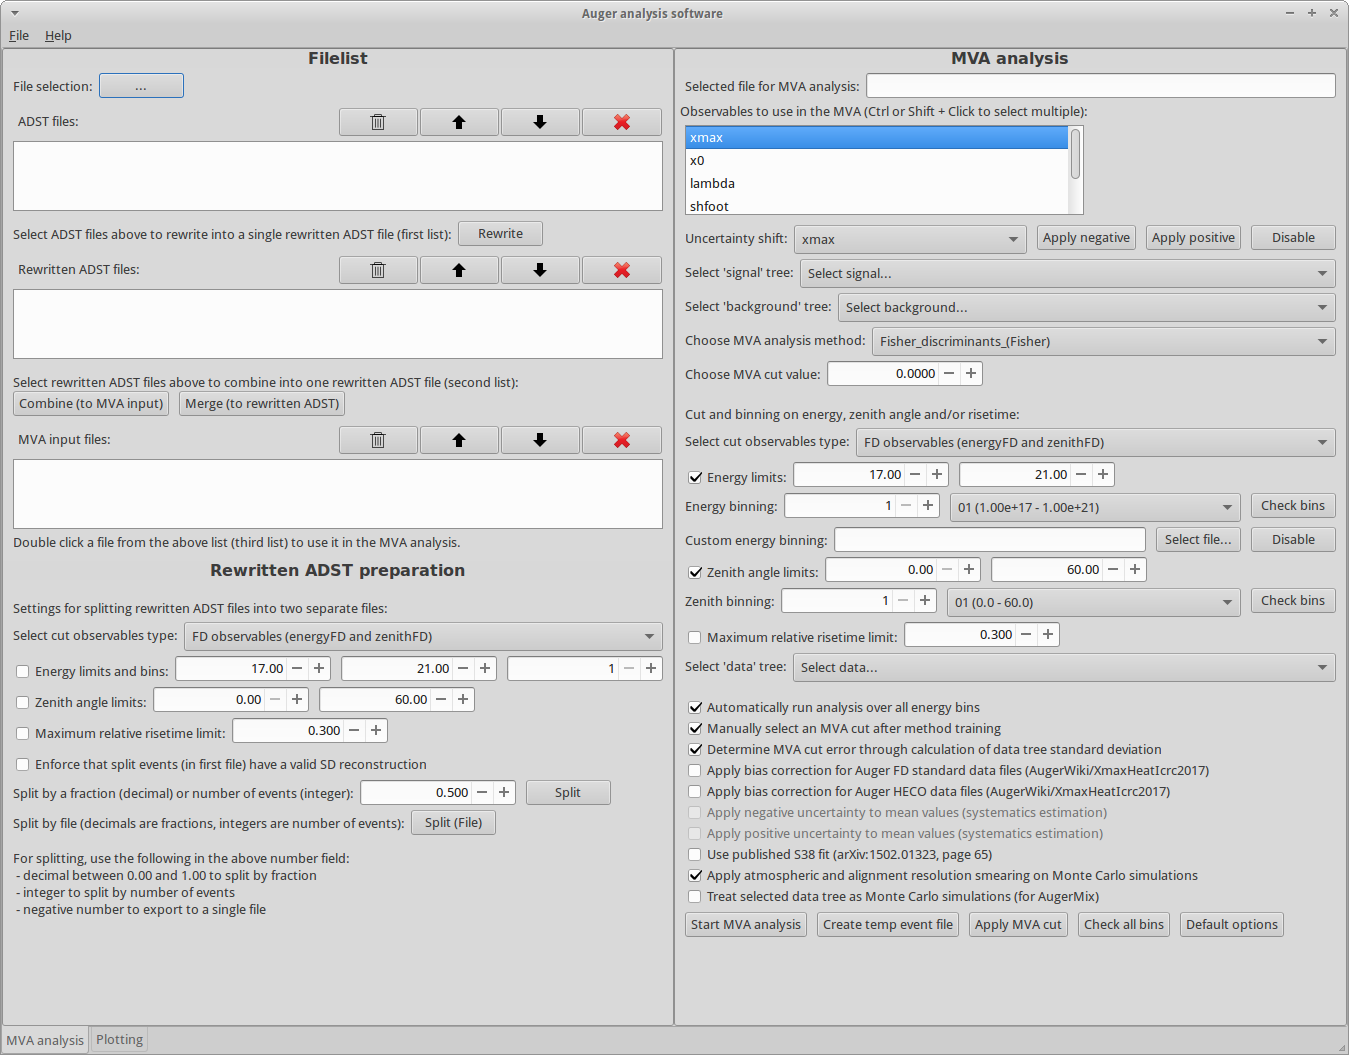
\includegraphics[width=0.94\textwidth]{figures/software_screenshot_1.png}}
\end{figure}
{\noindent}The analysis part of the interface is split into three different parts:
\begin{itemize}
\item[$\bullet$] \textbf{Filelist:} Handles opening of input files, which can be either Pierre Auger Observatory created ADST files (reconstructions from Offline) or the rewritten ADST files created with this software.
\item[$\bullet$] \textbf{Rewritten ADST preparation:} Handles operations on input files that enable to create precise data sets (smaller simulation samples, mixed simulation samples,\dots).
\item[$\bullet$] \textbf{MVA analysis:} Holds all options regarding the MVA analysis. This includes observables, signal/background samples, MVA methods, data binning and other options.
\end{itemize}
The \textbf{Filelist} part has an input file selector at the top, which passes input files through a check in order to determine their structure (handled by \texttt{SelectMvaFile} and \texttt{CheckFormat} functions in \texttt{./src/file\_operations.cpp}). Valid selected files are then correctly displayed in one of the three listboxes: Top for ADST files, middle for rewritten ADST files and bottom for completely prepared MVA input files. The four buttons above each listbox can be used for ordering or removing listed files. Note that in some listboxes it is possible to select multiple files, by holding down \texttt{Ctrl} or \texttt{Shift} and selecting them.\\
Rewritten ADST files are created by selecting files in the top listbox and using the button \texttt{Rewrite}. This extracts observables needed for further analysis, which are listed in \texttt{./input/observables.txt}. The rewriting process is handled by functions \texttt{StartRewrite} in \texttt{./src/connect\_functions.cpp} and the code in files \texttt{./src/adst\_mva.cpp} and \texttt{./src/calc\_observables.cpp}. In order for rewriting of new observables to work correctly, they need to be added in \linebreak\texttt{./src/calc\_observables.cpp}. Adding new observables is described in Chapter \ref{ch:add-obs}.\\
The middle listbox is used for either merging rewritten ADST files into single rewritten ADST files (for example merging different primary particle simulations for a mixed composition) or combining rewritten ADST files into MVA input files. These MVA input files will then typically hold at least three ROOT trees -- one for signal, one for background and one for data. The structure of these files is displayed on the figure below.
\begin{figure}[H]
\centerline{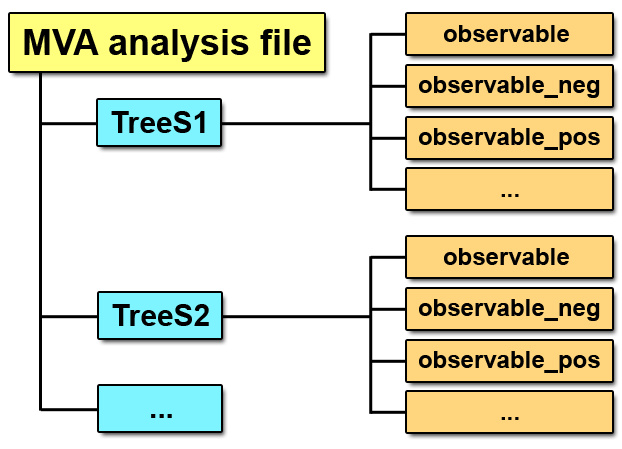
\includegraphics[width=0.40\textwidth]{figures/file_structure.png}}
\end{figure}
{\noindent}The bottom listbox is only there to open MVA input files. Double-clicking a file on this list selects it as the current input to the MVA analysis.\\
\\
The \textbf{Rewritten ADST preparation} part can be used to do additional preparations on rewritten ADST files. This includes binning in energy, limiting the zenith angle and selecting the maximal relative risetime (only comes into play when using obsevable \texttt{risetimerecalc}). For example, this can be used, when we need a precise mass composition of simulation files by setting a number of events in each file. It can also be used to split a simulation set into two parts, for instance when creating MVA training and cross-validation sets. The split can be set as a fraction (using a decimal between 0 and 1) or as the number of events that will appear in the first file (1 or larger). If the splitting fraction is set to a negative number, all events will be filtered according to the settings and exported into a single file (useful for just binning in energy or limiting the zenith angle). The setting to enforce a valid SD reconstruction in the first file is there to make sure all observables have been correctly reconstructed. This helps, when we want a precise mass composition for mixed composition samples. The difference between \texttt{Split} and \texttt{Split (File)} is that the first obeys the fraction or number of events entered in the number field, while the second uses a file with splitting instructions. This file needs to have the same number of lines as the number of selected rewritten ADST files. Each line can hold a decimal number (between 0 and 1) to set fractions or an integer to set the number of events. The files will then sequentially check each line and perform the splitting automatically. In case a specific energy binning structure is needed, use custom energy binning in the MVA analysis part.\\
\\
The \textbf{MVA analysis} part is the main part of this software and takes care of setting up and running the MVA analysis. The currently selected file is displayed in the top entry. In the listbox we can select observables that will be used as input features in the MVA analysis. Observables that are already included in the program are described in Chapter \ref{ch:observables}. The uncertainty shift setting is used to individually apply systematic uncertainties to observables in order to estimate the final systematic uncertainty of the analysis. Instructions for systematic uncertainty shifts need to be added to the \texttt{./src/mva\_analysis.cpp} file as described in Chapter \ref{ch:uncert}. The signal and background trees set training samples that the MVA analysis will try to separate according to the selected MVA method. All instructions for MVA methods are taken from the \texttt{./input/mva\_options.txt} input file. The setting for the MVA cut value is currently only a holder for eventual event-by-event identification and is automatically or manually selected during the analysis as the cut for best separation between signal and background. Settings on binning and limits give the possibility to split the MVA analysis based on energy and zenith angle on-the-fly. The selection of the data tree is typically the sample we wish to determine mass composition for (either mock data or real data). Important to note is that some observables (for example \texttt{deltas38} and \texttt{deltarisetime}) are always transformed using the selected data tree. The additional settings are:
\begin{itemize}
\item[$\bullet$] \emph{Automatically run analysis over all energy bins:}\\As the description suggests, this automatically runs the analysis over all selected energy bins. Note that this only works when we have a single MVA method selected.
\item[$\bullet$] \emph{Manually select an MVA cut after method training:}\\In case we wish to manually set the MVA cut value (mostly a holder for future event-by-event identification) after separation strength is known.
\item[$\bullet$] \emph{Determine MVA cut error through calculation of data tree standard deviation:}\\Currently only a holder for when statistical uncertainties can be determined directly from the MVA analysis. At the moment statistical uncertainties are handled by distribution fitting.
\item[$\bullet$] \emph{Apply bias correction for Auger FD standard data files (AugerWiki/XmaxHeatIcrc2017):}\\Apply bias corrections to the selected data tree according to the FD standard data approach, as described in \cite{CompositionAugerWiki}.
\item[$\bullet$] \emph{Apply bias correction for Auger HECO data files (AugerWiki/XmaxHeatIcrc2017):}\\Apply bias corrections to the selected data tree according to the HECO data approach, as described in \cite{CompositionAugerWiki}.
\item[$\bullet$] \emph{Use published S38 fit (arXiv:1502.01323, page 65):}\\When converting observable $S_{1000}$ into $\Delta S_{38}$ instead use the previously published fitting function values, presented in \cite{paoDesignReport}.
\item[$\bullet$] \emph{Apply atmospheric and alignment resolution smearing on Monte Carlo simulations:}\\Apply the smearing and bias corrections for Monte Carlo simulation samples, as described in \cite{xmaxMoments,xmaxUnger}. Note that smearing only works for Hybrid of FD data.
\item[$\bullet$] \emph{Treat selected data tree as Monte Carlo simulations (for AugerMix):}\\Perform Monte Carlo corrections on the selected data tree. Otherwise it is assumed that the data tree has real data selected.
\end{itemize}

{\noindent}Moving to the \texttt{Plotting} tab in the bottom left, we get to the plotting and distribution fitting part of the program:
\begin{figure}[H]
\centerline{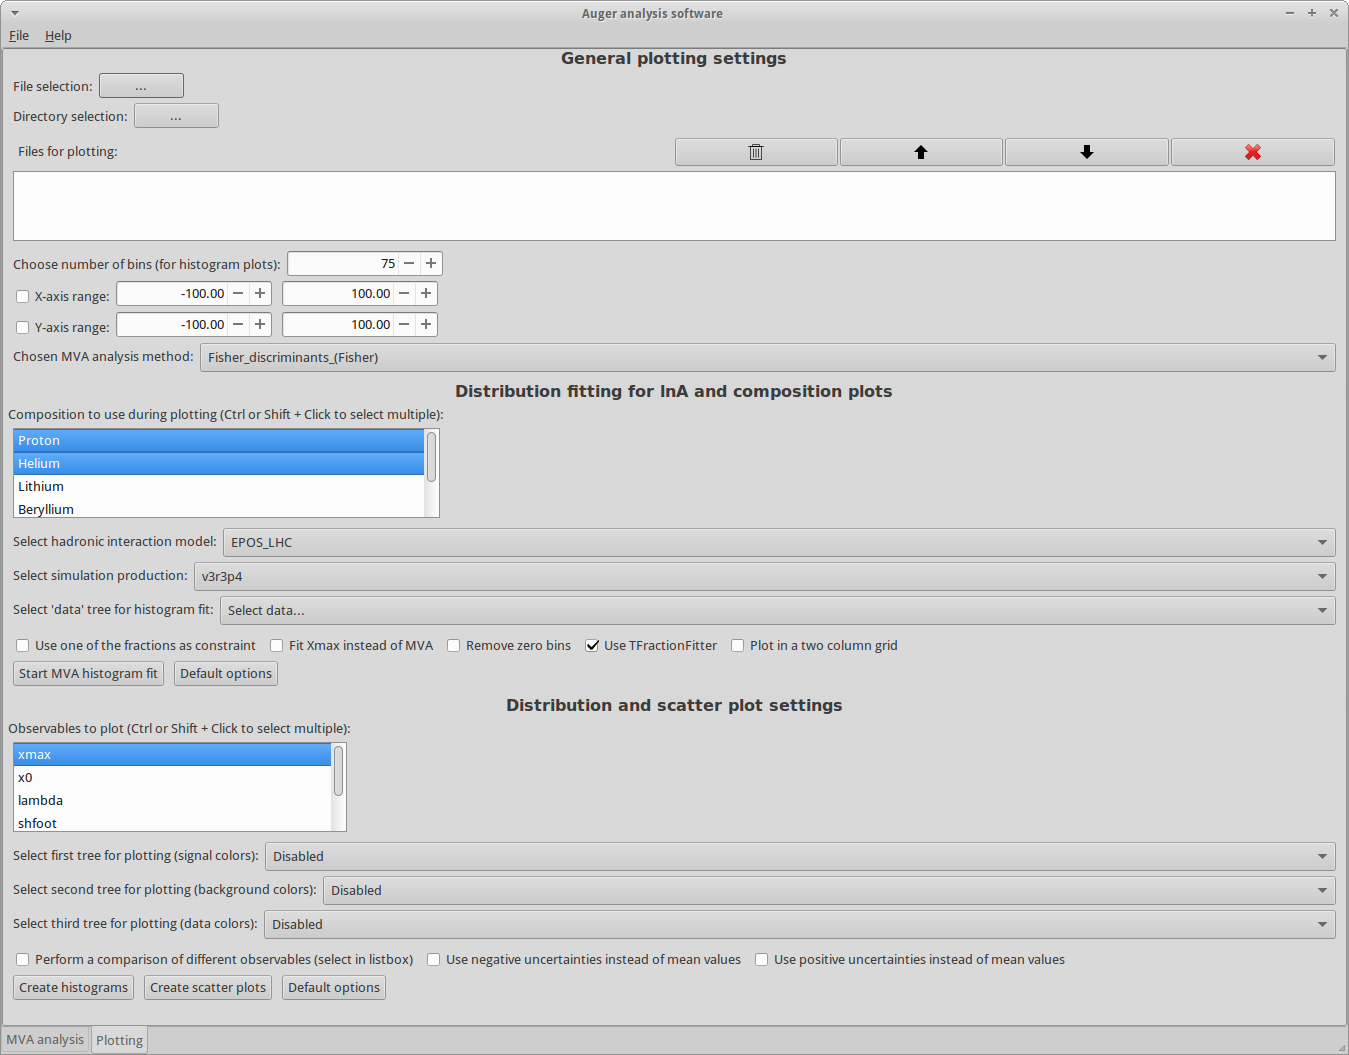
\includegraphics[width=0.94\textwidth]{figures/software_screenshot_2.png}}
\end{figure}
{\noindent}The plotting part of the interface is split into three different parts:
\begin{itemize}
\item[$\bullet$] \textbf{General plotting settings:} Handles opening of MVA analysis output files, which are ROOT files similar in structure to MVA input files, but with an added MVA variable distribution.
\item[$\bullet$] \textbf{Distribution fitting for lnA and composition plots:} Holds options for performing a distribution fitting procedure and extract elemental fractions from simulations. The complete fitting procedure is described in Chapter \ref{ch:distrib-fit}.
\item[$\bullet$] \textbf{Distribution and scatter plot settings:} Holds options for plotting distributions of any variable or scatter plots of a collection of them. It is able to plot up to three data sets on a single plot.
\end{itemize}
The \textbf{General plotting} part has an input file or input directory selector at the top, which makes it possible to open MVA analysis output files. There are also a range of settings that will be used universaly for any plot created by this program. The number of bins sets the binning structure, which applies to both distribution fitting and just plotting variable distributions. X-axis and Y-axis ranges can force all plots to use specific ranges, but are currently not implemented in the plotting procedure. The MVA method setting ensures that any naming and ranges are correct for the output MVA variable.\\
\\
The \textbf{Distribution fitting} part performs the distribution fitting procedure described in Chapter \ref{ch:distrib-fit}. In the listbox, we are able to select the composition mix that will be used for determining the mass composition. This composition must also be connected to the simulation trees that are in the MVA output file. Currently, the composition is setup in order to use this software directly with the Napoli shower library \cite{napoli}, which contains proton, helium, oxygen and iron as primary particles. The following settings choose the hadronic interaction model, data type and data tree we have used. The hadronic interaction model is the model used during event simulation and can be set in order to include previously published results \cite{xmaxICRC2017,xmaxDistFitPRD2014,deltaMethod} to composition plots. Using \texttt{None} will only show the results produced by this MVA analysis software. The simulation production just selects the Napoli library production we have used. The data tree can be the same as the data tree during the MVA analysis step, but we can also select the cross-validation or mock data sets. The remaining options are:
\begin{itemize}
\item[$\bullet$] \emph{Use one of the fractions as constraint:}\\Instead of leaving the constraint
$$
\displaystyle\sum_{i=1}^{N} f_i = 1,
$$
up to the fitting approach, force one of the elemental fractions $f_i$ to obey this constraint. For fitting with \texttt{TFractionFitter} this option can be disabled.
\item[$\bullet$] \emph{Fit Xmax instead of MVA:}\\Instead of using the output MVA variable distribution, use the depth of shower maximum $X_{\textrm{max}}$ for the distribution fitting procedure. For further development of the software, this will be extended to use any observable.
\item[$\bullet$] \emph{Remove zero bins:}\\During distribution fitting, all distribution bins are considered in the fit, even if they are zero. Enabling this setting removes distribution bins that have zero values from the fit.
\item[$\bullet$] \emph{Use TFractionFitter:}\\Use the distribution fitting approach \texttt{TFractionFitter} \cite{tfractionfitter} with maximum likelihood instead of the typical Minuit with $\chi^2$.
\item[$\bullet$] \emph{Plot in a two column grid:}\\The combined elemental fraction plot places all elements in the composition in a column on one image. The two column grid splits this into two columns. Note that due to the restrictions of ROOT and the display size, the two column grid image might have worse quality.
\end{itemize}
The \textbf{Distribution and scatter plot} part plots distributions or scatter plots of observables in order to make comparisons. In the listbox, we can select between all observables, including the output MVA variable. We can then select up to three different trees from the output MVA file, taking signal colors (blue), background colors (red) or data colors (black). The following options give some additional flexibility:
\begin{itemize}
\item[$\bullet$] \emph{Perform a comparison of different observables (select in listbox):}\\Instead of creating a normal plot, make a comparison between different observables from a single tree.
\item[$\bullet$] \emph{Use negative uncertainties instead of mean values:}\\Use mean values with added negative uncertainties instead of plotting mean values in the histogram or scatter plot.
\item[$\bullet$] \emph{Use positive uncertainties instead of mean values:}\\Use mean values with added positive uncertainties instead of plotting mean values in the histogram or scatter plot.
\end{itemize}

\section{Handling uncertainties} \label{ch:uncert}

\section{Distribution fitting procedure} \label{ch:distrib-fit}
MVA and individual observable distribution fitting is carried out by combining a mixture of primary elements into a simulation distribution
\begin{equation}\label{eq:simhistSum}
H_{\textrm{sim}} = \displaystyle\sum_{i=1}^{N}{f_i\, H_i},
\end{equation}
where $N$ is the number of elements in the mixture, $f_i$ are fractions of individual elements and $H_i$ are distributions of individual elements. The resulting distribution $H_{\textrm{sim}}$ is then fitted to the data distribution $H_{\textrm{data}}$. 
%\begin{equation}\label{eq:fractionSum}
%\displaystyle\sum_{i=1}^{N}{f_i} = 1.
%\end{equation}
%However, this approach did not bring satisfying fits, because distributions are finite and $\chi^2$ fits are primarily used on continuous distributions. This is especially apparent at the highest energy range, where the number of Pierre Auger data events is low.
Instead of using a $\chi^2$ fitting procedure, a maximum likelihood fitting approach was used through the TFractionFitter fitting package \cite{tfractionfitter} included in the ROOT framework. Specifically designed for fitting finite distributions with Poissonian statistics \cite{finiteMCfitting}, it naturally satisfies the normalization condition
\begin{equation}
\displaystyle\sum_{i=1}^{N}{f_i} = 1
\end{equation}
and limits elemental fractions to a $[0,1]$ range. The fitting procedure does not only enable MVA variable distribution fitting, but distribution fitting on any single observable. This skips the MVA analysis and tries to perform a distribution fit, with the same approach as described above. Fig. \ref{fig:distFit} shows the fitting procedure on MVA variable and $X_{\textrm{max}}$ distributions for a single energy bin.
%
\begin{figure}[!h]
\centering
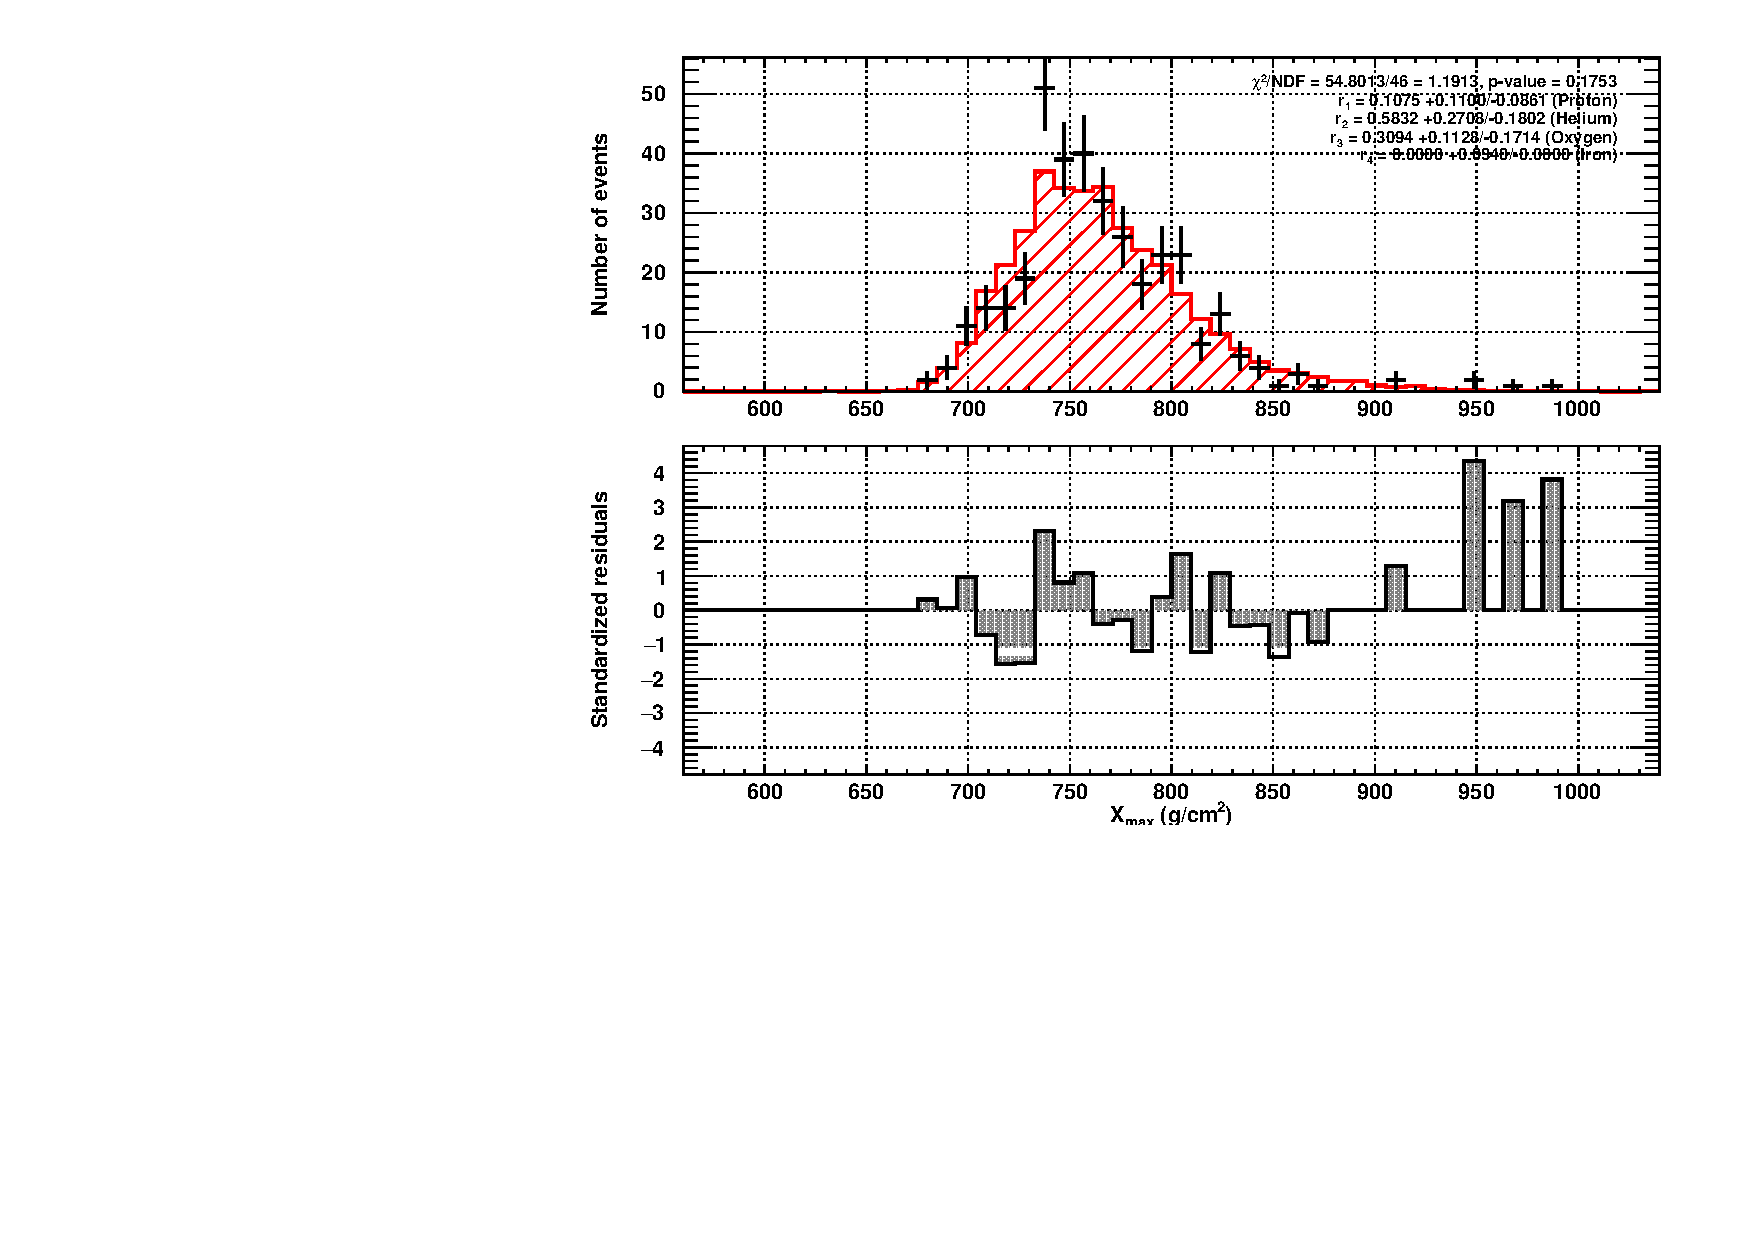
\includegraphics[width=0.494\textwidth,trim={0.9cm 0.0cm 0.8cm 0.2cm},clip]{figures/dist_fit_example_xmax.pdf}
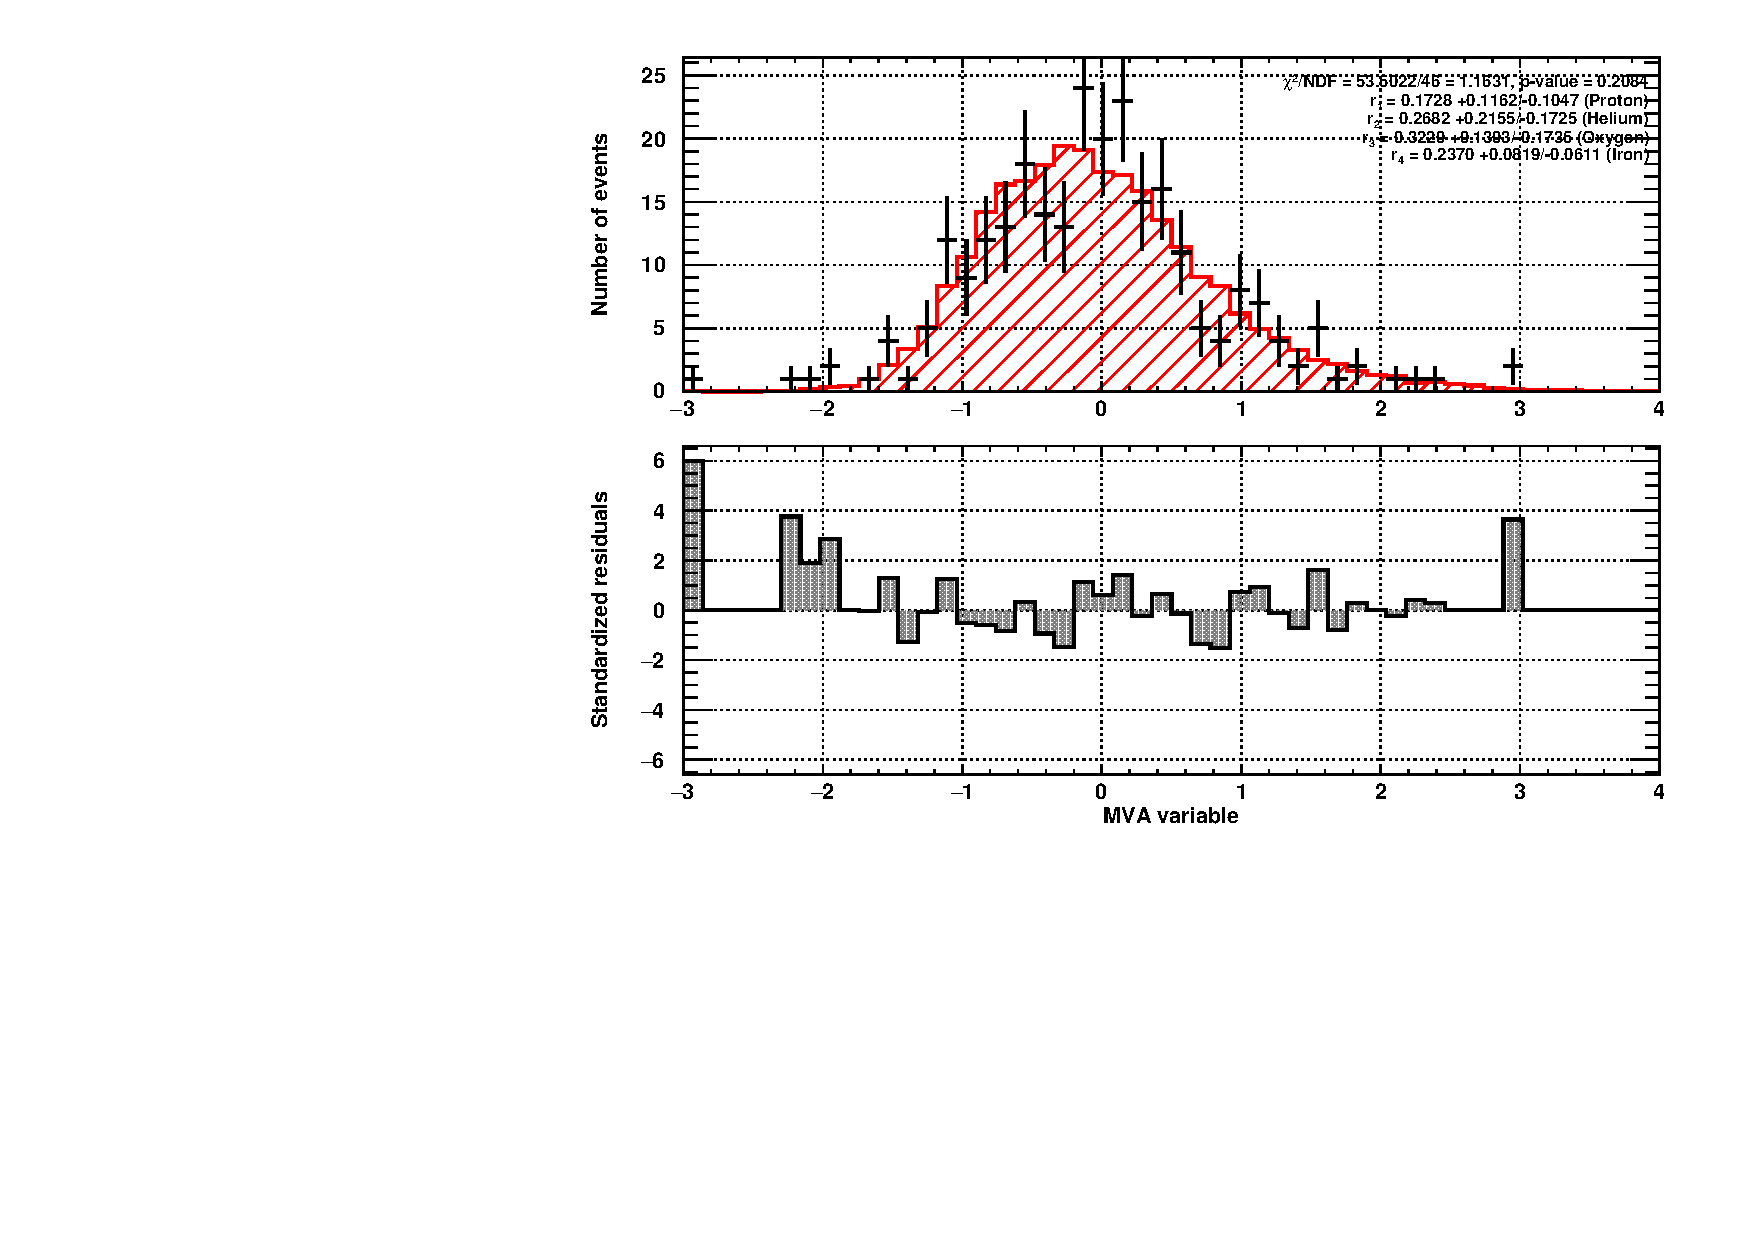
\includegraphics[width=0.470\textwidth,trim={1.8cm 0.0cm 0.8cm 0.2cm},clip]{figures/dist_fit_example_mva.pdf}
\caption{Example of distribution fits for $X_{\textrm{max}}$ (left) and MVA variable from a Fisher analysis (right). A four elemental composition $H_{\textrm{sim}}$ (red histogram) is fit onto a data distribution $H_{\textrm{data}}$ (black points) using a maximum likelihood fitting approach. Bottom panels show standardized residuals ($R_i = \frac{n_i - m_i}{\sqrt{n_i}}$) between data and simulations.} \label{fig:distFit}
\end{figure}
%
The fitting procedure returns elemental fractions for all included elements in the composition.

\section{Important input files}
Any important input files, through which the user can adjust or change input settings, are located in the \texttt{./input} folder. The following are some of these files:
\begin{itemize}
\item[$\bullet$] \textbf{MVA method options:}\\Input file with instructions for each of the included MVA methods from the TMVA package (\texttt{./input/mva\_options.txt}). The descriptive name will appear in the \texttt{Choose MVA analysis method} dropdown menu, while the method name is the name TMVA recognizes as an MVA method. Options for each of these methods can be adjusted, according to the TMVA documentation \cite{tmvadocument}. The file \texttt{./input/mva\_options.txt} must not be renamed in order for this to work!
\item[$\bullet$] \textbf{Observables file:}\\Input file with all observables we wish to extract from the ADST file and use in the MVA analysis (\texttt{./input/observables.txt}). The observable name appears in the observables listbox, while the selection sets the default selection of observables in the listbox. Note that the observable name must not include any whitespaces, because these are also used while naming output plots. Minimum and maximum limits are only used during plotting, where these two values are used to set limits for the appropriate axis. Axis labels give a description of the observable, which will be used during plotting. The file \texttt{./input/observables.txt} must not be renamed in order for this to work!
\item[$\bullet$] \textbf{Custom energy binning file:}\\Example of a custom energy binning input file \\(\texttt{./input/custom\_energy\_bins.txt}). The two columns determine low and high values of each energy bin as shown in this example:
\begin{lstlisting}[language=bash]
  18.5   18.6
  18.6   18.7
  18.7   18.8
  18.8   18.9
  18.9   19.0
  19.0   19.1
  19.1   19.2
  19.2   19.3
  19.3   19.4
  19.4   19.5
  19.5   20.0
\end{lstlisting}
This file can be selected using the \texttt{Select file...} button in the custom energy binning section of the MVA analysis part of the GUI.
\item[$\bullet$] \textbf{Splitting instructions file:}\\Example of a file, which sets instructions on how to automatically split multiple files. This is done through the \texttt{Split (File)} button in the Rewritten ADST preparation part of the GUI. Each line must include the number of events that will be saved to the first output file as shown in this example:
\begin{lstlisting}[language=bash]
  476
  326
  89
  28
  33
  28
  1
  22
  0
  7
  0
\end{lstlisting}
From this example, we have a total of 11 lines, which means this will sequentially split 11 selected input files automatically. When setting the splitting to 0, all events will be written to the second output file. Both output files will appear in the same folder as the input file, with an addition of \texttt{split1} or \texttt{split2} to their names, in order to separate them.
\item[$\bullet$] \textbf{Previously published results files:}\\In order to plot previously published results in addition to the results created through the MVA analysis method, some input files must describe them:
	\begin{itemize}
	\item[--] File \texttt{./input/fractions\_icrc17.txt} includes elemental fractions reported in \cite{xmaxICRC2017} and can be found in \cite{CompositionAugerWiki}.
	\item[--] Files \texttt{./input/lnA\_moments\_icrc2017\_*.txt} include $\left<\ln A\right>$ values reported in \cite{xmaxICRC2017} and can be found in \cite{CompositionAugerWiki}.
	\item[--] Files \texttt{./input/lnA\_moments\_prd2014\_*.txt} include $\left<\ln A\right>$ values reported in \cite{xmaxDistFitPRD2014} and can be found in \cite{UngerComposition}.
	\item[--] Files \texttt{./input/lnA\_moments\_sd*.txt} include $\left<\ln A\right>$ values reported in \cite{deltaMethod} and can be found in \cite{DeltaComposition}.
	\end{itemize}
Note that all of these input files have to be structured by the user accordingly or the plotting code needs to be adjusted. Functions handling the reading of these files are \texttt{ReadFracResultsFD}, \texttt{ReadLnaResultsFD} and \texttt{ReadLnaResultsSD}, all located in file \texttt{./src/mva\_fit\_histogram.cpp}.
\end{itemize}

\chapter{Extensive air shower observables} \label{ch:observables}
{\noindent}This chapter describes the extensive air shower observables already included in the program and gives instructions on how to add new observables. Each of the descriptions also explains how it was extracted from the ADST file structure of Offline. Note that \texttt{fFile} denotes the reconstructed ADST file (\texttt{RecEventFile}) and \texttt{fRecEvent} denotes an event in this file (\texttt{RecEvent}). The rewriting and extraction of individual observables is handled in files \texttt{./src/adst\_mva.cpp} and \texttt{./src/calc\_observables.cpp}.

\section{Observable descriptions}

\subsection{\texttt{xmax} -- Depth of shower maximum}
The depth of shower maximum $X_{\textrm{max}}$ is the depth at which the extensive air shower reaches its maximum number of particles. This occurs due to energy loss of secondary particles, which at the critical energy of ${\sim}\unit[]{GeV}$ are less likely to produce new particles. The maximum clearly appears in measurements of UV light coming from the interaction of secondaries in the extensive air shower and nitrogen molecules. The so-called longitudinal profile of the shower (energy loss along the shower axis) is then fitted with a Gaisser-Hillas function
\begin{equation}\label{eq:gaisserHillas}
f_{\textrm{GH}}(X) = \left(\frac{\diff E}{\diff X}\right)_{\textrm{max}}\cdot \left(\frac{X - X_0}{X_{\textrm{max}} - X_0}\right)^{\frac{X_{\textrm{max}} - X_0}{\lambda}}\, \me^{\frac{X_{\textrm{max}} - X}{\lambda}},
\end{equation}
where $X$ is the depth along the shower axis, and $\lambda$, $X_0$, $X_{\textrm{max}}$ and $\left(\frac{\diff E}{\diff X}\right)_{\textrm{max}}$ are shape parameters of the shower. From the ADST structure, the depth of shower maximum measured by an FD building (denoted with \texttt{eye}) can be accessed with
\begin{lstlisting}[language=C++]
  vector<FDEvent> acteyes;
  acteyes = fRecEvent->GetFDEvents();
  xmax = (acteyes[eye].GetFdRecShower()).GetXmax();
\end{lstlisting}
The reading and extraction of this observable is handled by function \texttt{GetXmax} in file \texttt{./src/calc\_observables.cpp}.

\subsection{\texttt{x0} -- First interaction depth}
$X_0$ describes the depth at which the initial interaction happened between the primary cosmic ray and an atmospheric molecule. This value depends on the simulation software and its atmospheric model, but is directly extracted from equation \eqref{eq:gaisserHillas}. From the ADST structure, the first interaction depth measured by an FD building (denoted with \texttt{eye}) can be accessed with
\begin{lstlisting}[language=C++]
  vector<FDEvent> acteyes;
  acteyes = fRecEvent->GetFDEvents();
  x0 = (acteyes[eye].GetFdRecShower()).GetX0();
\end{lstlisting}
The reading and extraction of this observable is handled by function \texttt{GetX0} in file \texttt{./src/calc\_observables.cpp}.

\subsection{\texttt{lambda} -- Gaisser-Hillas fitting parameter $\lambda$}
Similarly to the previous two observables, $\lambda$ is also a fitting parameter of the longitudinal profile and is directly extracted from equation \eqref{eq:gaisserHillas}. From the ADST structure, the $\lambda$ parameter measured by an FD building (denoted with \texttt{eye}) can be accessed with
\begin{lstlisting}[language=C++]
  vector<FDEvent> acteyes;
  acteyes = fRecEvent->GetFDEvents();
  lambda = (acteyes[eye].GetFdRecShower()).GetLambda();
\end{lstlisting}
The reading and extraction of this observable is handled by function \texttt{GetLambda} in file \texttt{./src/calc\_observables.cpp}.

\subsection{\texttt{shfoot} -- Early development of the extensive air shower}
The shower foot is an experimental observable which treats the longitudinal profile of a shower similarly as risetime determines the early deposit of energy from SD photomultiplier signals. The idea of this variable is to determine the depth at which the longitudinal profile reaches $10\%$ of the maximum of the cumulative longitudinal profile. As such, the observable could be able to predict the early development of an extensive shower, which should be larger for heavier primary particles. Note, however, that this observable has not been thoroughly tested and should not be used, unless more detailed analysis is performed.\\
The shower foot has a default fractional value of $\texttt{showerlimit} = 0.1$, where it is estimated. For each of the FD buildings (denoted with \texttt{eye}), we first extract the longitudinal development of the shower with
\begin{lstlisting}[language=C++]
  vector<FDEvent> acteyes;
  acteyes = fRecEvent->GetFDEvents();
  vector<double> *slantDepth = new vector<double>;
  vector<double> *profiledEdX = new vector<double>;
  vector<double> *profiledEdXerr = new vector<double>;
  *slantDepth = (acteyes[eye].GetFdRecShower()).GetDepth();
  *profiledEdX = (acteyes[eye].GetFdRecShower()).GetEnergyDeposit();
  *profiledEdXerr = (acteyes[eye].GetFdRecShower()).GetEnergyDepositError();
\end{lstlisting}
This profile is then converted into its cumulative distribution with:
\begin{lstlisting}[language=C++]
  double x = 0., xerr = 0.;
  vector<double> xfoot;
  vector<double> yfoot;
  vector<double> yerrfoot;
  for(int i = 0; i < slantDepth->size(); i++)
  {
    x += profiledEdX->at(i);
    xerr += profiledEdXerr->at(i);
    xfoot.push_back(slantDepth->at(i));
    yfoot.push_back(x);
    yerrfoot.push_back(xerr);
  }
\end{lstlisting}
Once we have this distribution, we simply determine the final shower foot value, when the cumulative distribution reaches the \texttt{shfootlimit} fraction of its maximum
\begin{lstlisting}[language=C++]
  for(int i = 0; i < yfoot.size(); i++)
  {
    if(yfoot[i] >= shfootlimit*(yfoot[yfoot.size()-1]))
    {
      // estimate the exact value between two points with linear interpolation
      // ...
      break;
    }
  }
\end{lstlisting}
The reading and extraction of this observable is handled by functions \texttt{CalculateShowerFoot} and \texttt{GetShowerFoot} in file \texttt{./src/calc\_observables.cpp}.

\subsection{\texttt{energySD} -- SD reconstructed primary energy}
This is the reconstructed energy as measured by the surface detector (SD). From the ADST structure, $E_{\textrm{SD}}$ can be accessed with
\begin{lstlisting}[language=C++]
  SdRecShower *sdrecshw;
  *sdrecshw = fRecEvent->GetSDEvent().GetSdRecShower();
  energySD = sdrecshw->GetEnergy();
\end{lstlisting}
The reading and extraction of this observable is handled by function \texttt{GetSdEnergy} in file \texttt{./src/calc\_observables.cpp}.

\subsection{\texttt{energyFD} -- FD reconstructed primary energy}
This is the reconstructed energy as measured by one of the FD buildings. From the ADST structure, $E_{\textrm{FD}}$ measured by an FD building (denoted with \texttt{eye}) can be accessed with
\begin{lstlisting}[language=C++]
  vector<FDEvent> acteyes;
  acteyes = fRecEvent->GetFDEvents();
  energyFD = (acteyes[eye].GetFdRecShower()).GetEnergy();
\end{lstlisting}
The reading and extraction of this observable is handled by function \texttt{GetFdEnergy} in file \texttt{./src/calc\_observables.cpp}.

\subsection{\texttt{nrmu} -- Number of muons at ground level}
For the time being, the number of muons at ground level is only determined through the simulated part of the shower. As such, any real data events will be missing this information. From the ADST structure, the number of muons can be accessed with
\begin{lstlisting}[language=C++]
  GenShower *genshw;
  genshw = fRecEvent->GetGenShower();
  nrmu = genshw->GetMuonNumber();
\end{lstlisting}
The reading and extraction of this observable is handled by function \texttt{GetNrMuons} in file \texttt{./src/calc\_observables.cpp}.

\subsection{\texttt{nrstations} -- Number of triggered stations}
This observable gives the number of SD stations that were triggered by an event. Each station is checked in order to see, if its signal is above the minimum VEM signal (\texttt{minSignal}), if it is not low gain saturated, if it is inside the limits for the distance from the shower axis (\texttt{limitDistance}), if its asymmetry corrected risetime has been calculated correctly and if its calculated uncertainty is positive. If the total number of stations tiggered by an event is lower than a predetermined limit of triggered stations for calculation of risetime (\texttt{minPoint}), this value will not be available. From the ADST structure, the number of triggered stations can be accessed with
\begin{lstlisting}[language=C++]
  vector<SdRecStation> actstations;
  actstations = fRecEvent->GetSDEvent().GetStationVector();
  int itemp;
  for(int i = 0; i < actstations.size(); i++)
  {
    if(actstations[i].IsCandidate())
    {
      /* --- Calculation of station risetime --- */
      bool btemp = true;
      if(actstations[i].GetTotalSignal() < minSignal) btemp = false;
      if(actstations[i].IsLowGainSaturated()) btemp = false;
      if( (actstations[i].GetSPDistance() < limitDistance[0]) || (actstations[i].GetSPDistance() > limitDistance[1]))
        btemp = false;
      if(risemean < 0.) btemp = false;
      if(riseerr < 0.) btemp = false;

      if(btemp)
        itemp++;
    }
  }

  if(itemp >= minPoints)
    nrstations = itemp;
\end{lstlisting}
The reading and extraction of this observable is handled by functions \texttt{SetStationValues} and \texttt{GetNrStations} in file \texttt{./src/calc\_observables.cpp}.

\subsection{\texttt{shwsize} -- SD signal at $\unit[1000]{m}$ from the shower axis}
This returns the SD signal at $\unit[1000]{m}$ from the shower axis as determined by the fit of the lateral distribution function
\begin{equation} \label{eq:ldfFunction}
S(r) = S_{1000}\, \left(\frac{r}{\unit[1000]{m}}\right)^{\beta}\cdot \left(\frac{r + \unit[700]{m}}{\unit[1700]{m}}\right)^{\beta + \gamma},
\end{equation}
where $r$ is the distance from the shower axis, $S_{1000}$ is the SD signal at $\unit[1000]{m}$ from the shower axis, and $\beta$ and $\gamma$ are the LDF fitting parameters. This observable is an indicator of the muonic content of a shower, since showers induced by heavier primaries typically have a larger muonic content and form a larger footprint on the surface detector. From the ADST structure, $S_{1000}$ can be accessed with
\begin{lstlisting}[language=C++]
  SdRecShower *sdrecshw;
  *sdrecshw = fRecEvent->GetSDEvent().GetSdRecShower();
  shwsize = sdrecshw->GetShowerSize();
\end{lstlisting}
Note that the function \texttt{GetS1000} is deprecated and \texttt{GetShowerSize} is used instead. The reading and extraction of this observable is handled by function \texttt{GetShowerSize} in file \texttt{./src/calc\_observables.cpp}.

\subsection{\texttt{deltas38} -- Relative SD signal}
$S_{1000}$ is however dependent on zenith angle, so it is reasonable to prepare a relative SD signal value ($\Delta S_{38}$), which will be independent of both distance from shower axis and the zenith angle. The calculation follows these steps:
\begin{itemize}
\item[1.] Scatter plots of station signal $S_{1000}$ versus zenith angle ($\sec \theta$) are plotted for a range of energy bins.
\item[2.] These are then fitted with a scaled constant intensity cut function $f_{\textrm{scale}}(\theta)$ in order to remove dependence of $S_{1000}$ on the zenith angle, and convert it to $S_{38}$.
\item[3.] When conversions to $S_{38}$ are finished for all energy bins, they are combined and fitted with a power law function.
\item[4.] The relative signal $\Delta S_{38}$ is calculated by determining the separation between $S_{38}$ of each event and the fitted power law function. Additionally, its uncertainty $\delta \Delta S_{38}$ is calculated through propagation of uncertainties.
\end{itemize}
$S_{1000}$ are divided into energy bins between $\unit[10^{18.5}]{eV}$ and $\unit[10^{20.0}]{eV}$. The binning step is selected to be $\log(E/\unit[]{eV}) = 0.1$, except for the final bin in Pierre Auger data events, which spans between $\unit[10^{19.5}]{eV}$ and $\unit[10^{20.0}]{eV}$. This has been selected in order to remedy the small amount of events at high energies, while still keeping as much information on simulations. Each of these subsets are then fitted with a scaled constant intensity cut function
\begin{equation}
f_{\textrm{scale}}(\theta) = S\, f_{\textrm{CIC}}(\theta) = S\, \left(1 + a x + b x^2 + c x^3\right),
\end{equation}
where $x$ is
\begin{equation}\label{eq:relativeS38}
x = \cos^2 \theta - \cos^2(38^{\circ}),
\end{equation}
and $S$, $a$, $b$ and $c$ are free fitting parameters. Parameter $S$ will not come into play for further conversion of $S_{1000}$, but it represents the average $S_{38}$ for the selected energy bin. The signal at $\unit[1000]{m}$ from the shower axis and at a reference zenith angle value of $38^{\circ}$ is then defined as
\begin{equation}\label{eq:s1000tos38}
S_{38} = \frac{S_{1000}}{f_{\textrm{CIC}}(\theta)}.
\end{equation}
As an alternative to removing zenith angle dependence by fitting $S_{1000}$ values, the previously published attenuation curve $f_{\textrm{CIC}}(\theta)$, with $a = 0.980\pm 0.004$, $b = -1.68\pm 0.01$ and $c = -1.30\pm 0.45$, can be used instead \cite{fcicICRC2013}. Once fits for all energy bins have been performed, all $S_{38}$ values are fitted with a power law function
\begin{equation}\label{eq:powerlawfit}
f_{38}(E_{\textrm{FD}}) = \left(\frac{E_{\textrm{FD}}}{A}\right)^{\rfrac{1}{B}},
\end{equation}
where $A$ and $B$ are free fitting parameters. As before, this fit can be replaced with previously published values of $A = \unit[(1.90\pm 0.05)\times 10^{17}]{eV}$ and $B = 1.025\pm 0.007$ from \cite{fcicICRC2013}. At this point, the power law fitting function is used as a reference for calculating $\Delta S_{38}$ values
\begin{equation}
\Delta S_{38} = S_{38} - f_{38}(E_{\textrm{FD}}).
\end{equation}
As opposed to other observables, this observable is calculated from SD station signals at $\unit[1000]{m}$ from the shower axis right before the MVA analysis step. This enables the user to select the data set, which will produce the reference zero value of the $\Delta S_{38}$ observable. The fitting is handled by function \texttt{SetDeltas} in file \texttt{./src/mva\_analysis.cpp}, while the conversion is handled by functions \texttt{ConvertToS38} and \texttt{ConvertToDeltaS38} in file \texttt{./src/observables.cpp}.

\subsection{\texttt{ldfbeta} -- Lateral distribution function fitting parameter $\beta$}
$\beta$ is a fitting parameter in the lateral distribution function and is directly extracted from equation \eqref{eq:ldfFunction}. From the ADST structure, $\beta$ can be accessed with
\begin{lstlisting}[language=C++]
  SdRecShower *sdrecshw;
  *sdrecshw = fRecEvent->GetSDEvent().GetSdRecShower();
  shwsize = sdrecshw->GetBeta();
\end{lstlisting}
The reading and extraction of this observable is handled by function \texttt{GetBeta} in file \texttt{./src/calc\_observables.cpp}.

\subsection{\texttt{curvature} -- The curvature of the shower front}
This observable describes the curvature of the shower front in units of $\unit[]{m^{-1}}$ as measured by the surface detector (SD). From the ADST structure, the curvature can be accessed with
\begin{lstlisting}[language=C++]
  SdRecShower *sdrecshw;
  *sdrecshw = fRecEvent->GetSDEvent().GetSdRecShower();
  curvature = sdrecshw->GetCurvature();
\end{lstlisting}
The reading and extraction of this observable is handled by function \texttt{GetCurvature} in file \texttt{./src/calc\_observables.cpp}.

\subsection{\texttt{risetime, risetimerecalc} -- SD risetime at $\unit[1000]{m}$ from the shower axis}
The SD risetime is the time it takes the cumulative SD station signal to get from 10\% to 50\% of its maximal value. It is an indicator of electromagnetic versus muonic content in a shower, since muons produce sharp peaks in the station signal (formed high in the atmosphere) and electromagnetic particles form the broad distribution (formed closer to the surface). Shorter risetimes are thus typically attributed to showers induced by heavier primary particles. Because risetime is dependent on the distance from the shower axis, one of the reference points is to perform a fit through all SD station risetimes in an event
\begin{equation}\label{eq:risetimeFit}
f(r) = \unit[40]{ns} + a\cdot r + b\cdot r^2
\end{equation}
and take the value at $\unit[1000]{m}$ from the shower axis. Important options for determining this observable are:
\begin{itemize}
\item[$\bullet$] \textbf{Range of valid SD station distances from the shower axis:}\\
Setting minimum and maximum distances for valid SD station risetime enables removal of stations that would cause biases or have problems due to detector sampling. The default value of the range is between $\unit[0]{m}$ and $\unit[1800]{m}$. The range used in \cite{deltaMethod} is however between $\unit[300]{m}$ and $\unit[1400]{m}$ for energies below $\unit[10^{19.6}]{eV}$, and $\unit[300]{m}$ and $\unit[2000]{m}$ for primary energies above $\unit[10^{19.6}]{eV}$.
\item[$\bullet$] \textbf{Minimum total SD station signal:}\\
The minimum SD station signal sets the threshold, which removes any stations with a low signal measurement. The default value of the threshold is $\unit[10]{VEM}$ ($\unit[]{VEM}$ is the Vertical-Equivalent-Muon unit and describes the signal produced by a muon passing the SD station vertically and through the station center). The threshold used in \cite{deltaMethod} reduces this to $\unit[5]{VEM}$ in order to not remove too many SD stations at lower energies.
\item[$\bullet$] \textbf{Including low-gain saturated stations:}\\
The SD signal is recorded in both the high-gain and low-gain channel. This is due to the large extent of signal sizes, when measuring extensive air showers. When the high-gain channel is saturated (signal is higher than the maximum of the ADC converter), analysis is performed on the low-gain channel. If the low-gain channel is saturated, the SD station is typically discarded from any further analysis.
\item[$\bullet$] \textbf{Evaluation distance:}\\
The evaluation or reference distance from the shower axis removes any dependency on distance from shower axis. Typically, the SD risetime value is selected at $\unit[1000]{m}$ from the shower axis.
\item[$\bullet$] \textbf{Minimum number of triggered stations:}\\
In order to perform a fit through triggered stations with equation \eqref{eq:risetimeFit}, a minimum number of triggered stations needs to be determined. Typically, an event is considered to be valid if at least 3 stations are triggered and do not fall outside of previous selections mentioned above.
\end{itemize}
The difference between the \texttt{risetime} and \texttt{risetimerecalc} observables is only in selected options. \texttt{risetime} uses the default options and can be accessed from the ADST structure with
\begin{lstlisting}[language=C++]
  SdRecShower *sdrecshw;
  *sdrecshw = fRecEvent->GetSDEvent().GetSdRecShower();
  risetime = sdrecshw->GetRiseTimeResults().GetRiseTime1000();
\end{lstlisting}
The reading and extraction of this observable is handled by function \texttt{GetRisetime} in file \texttt{./src/calc\_observables.cpp}.\\
\texttt{risetimerecalc}, on the other hand, repeats the reconstruction of SD risetime, but uses options from \cite{deltaMethod}. The reading and extraction of this observable is handled by functions \texttt{CalculateRisetime} and \texttt{GetRisetime} in file \texttt{./src/calc\_observables.cpp}.

\subsection{\texttt{deltarisetime} -- Relative SD risetime}
A further complication arises, when checking the zenith angle dependence of SD station risetime. Due to that, it is reasonable to prepare a relative SD risetime value ($\Delta_R$), which will be independent of both distance from shower axis and the zenith angle.
The conversion uses a similar treatment to the $\Delta_s$ method introduced in \cite{deltaMethod}. During the conversion, the following steps are made:
\begin{itemize}
\item[1.] Station risetimes with high-gain saturation are treated differently, because they introduce a bias that is visible while fitting.
\item[2.] Scatter plots of station risetime $t_{1/2}$ versus distance $r$ are plotted for a range of zenith angle bins at a reference energy bin (between $\unit[10^{18.9}]{eV}$ and $\unit[10^{19.1}]{eV}$). The reference energy bin is slightly larger than in \cite{deltaMethod}, because it was primarly prepared for the hybrid dataset, which has smaller statistics. The energy reference bin and zenith angle binning (\texttt{binLimit}) is defined in the \texttt{SetDeltas} function of file \texttt{./src/mva\_analysis.cpp}. This zenith angle binning removes the dependence of risetime on zenith angle.
\item[3.] Both sets of station risetimes (high-gain saturated and non-saturated) are separately fitted with benchmark functions. This removes the dependence of risetime on distance from the shower axis.
\item[4.] SD station relative risetimes $\Delta_i$ are calculated by determining the separation between the station risetime and the appropriate benchmark function inside the appropriate zenith angle bin.
\item[5.] Event-wide $\Delta_R$ and its uncertainty $\delta \Delta_R$ are calculated from the average of station relative risetimes.
\end{itemize}
The benchmark fitting functions are selected to be
\begin{equation}\label{eq:HGbench}
t_{1/2}^{\textrm{bench},\textrm{HG-sat}} = \unit[40]{ns} + \sqrt{A^2 + B^2\, r^2} - A,
\end{equation}
for a fit to high-gain saturated SD station risetimes and
\begin{equation}\label{eq:normalbench}
t_{1/2}^{\textrm{bench}} = \unit[40]{ns} + M\, (\sqrt{A^2 + B^2\, r^2} - A),
\end{equation}
for a fit to non-saturated SD station risetimes. During the fitting procedure, high-gain saturated risetimes are fitted first, because they typically have a smaller spread. The two fitting parameters $A$ and $B$ are then fixed for the fit to non-saturated risetimes, where the only free parameter $M$ describes the bias. With benchmark functions set in all zenith angle bins, we can now calculate the station relative risetime $\Delta_i$, by determining the separation of $t_{1/2}$ to the appropriate benchmark function
\begin{equation}
\Delta_i = t_{1/2} - t_{1/2}^{\textrm{bench}}.
\end{equation}
Calculation of $\Delta_i$ again differs from the approach used in \cite{deltaMethod}, because low statistics of hybrid data makes the estimation of $\sigma_{1/2}$ difficult. Finally, $\Delta_R$ is simply the average of all stations relative risetimes involved in a single event
\begin{equation}
\Delta_R = \frac{1}{N} \displaystyle\sum_{i = 1}^{N} \Delta_i,
\end{equation}
where $N$ is the number of triggered stations in a shower event. All uncertainties on $S_{38}$ and $\Delta S_{38}$ are calculated through uncertainty propagation.\\
As opposed to other observables, this observable is calculated from SD station risetimes right before the MVA analysis step. This enables the user to select the data set, which will produce the reference zero value of the $\Delta_R$ observable. The fitting is handled by function \texttt{SetDeltas} in file \texttt{./src/mva\_analysis.cpp}, while the conversion is handled by function \texttt{ConvertToDelta} in file \texttt{./src/observables.cpp}.

\subsection{\texttt{aop} -- Area-over-peak}
The area-over-peak (AoP) is an observable that checks the area under the photomultiplier signal trace versus the peak value of the same trace. It is an indicator of electromagnetic versus muonic content in a shower, since muons produce sharp peaks in the station signal (formed high in the atmosphere) and electromagnetic particles form the broad distribution (formed closer to the surface). Showers with higher electromagnetic content will have a larger area under the signal, thus exhibiting a larger AoP value. The area (charge) and peak value of a specific photomultiplier in each of the SD stations are determined with
\begin{lstlisting}[language=C++]
  double charge, peak, aop;
  vector<SdRecStation> stationVector =
    fRecEvent->GetSDEvent().GetStationVector();
  for(int i = 0; i < stationVector.size(); i++)
  {
    if(stationVector[i].IsCandidate())
    {
      // loop over photomultipliers
      for(int j = 1; j <= 3; j++)
      {
        charge = stationVector[i].GetCharge(j);
        peak = stationVector[i].GetPeak(j);
	aop = charge/peak;
      }
    }
  }
\end{lstlisting}
Individual photomultiplier AoP values are then summed together into a mean AoP value, depending on the number of active photomultipliers and active SD stations in an event. The reading and extraction of this observable is handled by functions \texttt{CalculateAoP} and \texttt{GetAoP} in file \texttt{./src/calc\_observables.cpp}.

\subsection{\texttt{zenithSD} -- SD reconstructed zenith angle}
This is the reconstructed zenith angle as measured by the surface detector (SD). From the ADST structure, $\theta_{\textrm{SD}}$ can be accessed with
\begin{lstlisting}[language=C++]
  SdRecShower *sdrecshw;
  *sdrecshw = fRecEvent->GetSDEvent().GetSdRecShower();
  zenithSD = sdrecshw->GetZenith();
\end{lstlisting}
The reading and extraction of this observable is handled by function \texttt{GetSdZenith} in file \texttt{./src/calc\_observables.cpp}.

\subsection{\texttt{azimuthSD} -- SD reconstructed azimuth angle}
This is the reconstructed azimuth angle as measured by the surface detector (SD). From the ADST structure, $\phi_{\textrm{SD}}$ can be accessed with
\begin{lstlisting}[language=C++]
  SdRecShower *sdrecshw;
  *sdrecshw = fRecEvent->GetSDEvent().GetSdRecShower();
  azimuthSD = sdrecshw->GetAzimuth();
\end{lstlisting}
The reading and extraction of this observable is handled by function \texttt{GetSdAzimuth} in file \texttt{./src/calc\_observables.cpp}.

\subsection{\texttt{zenithFD} -- FD reconstructed zenith angle}
This is the reconstructed zenith angle as measured by one of the FD buildings. From the ADST structure, $\theta_{\textrm{FD}}$ measured by an FD building (denoted with \texttt{eye}) can be accessed with
\begin{lstlisting}[language=C++]
  vector<FDEvent> acteyes;
  acteyes = fRecEvent->GetFDEvents();
  zenithFD = (acteyes[eye].GetFdRecShower()).GetZenith();
\end{lstlisting}
The reading and extraction of this observable is handled by function \texttt{GetFdZenith} in file \texttt{./src/calc\_observables.cpp}.

\subsection{\texttt{azimuthFD} -- FD reconstructed azimuth angle}
This is the reconstructed azimuth angle as measured by one of the FD buildings. From the ADST structure, $\phi_{\textrm{FD}}$ measured by an FD building (denoted with \texttt{eye}) can be accessed with
\begin{lstlisting}[language=C++]
  vector<FDEvent> acteyes;
  acteyes = fRecEvent->GetFDEvents();
  azimuthFD = (acteyes[eye].GetFdRecShower()).GetAzimuth();
\end{lstlisting}
The reading and extraction of this observable is handled by function \texttt{GetFdAzimuth} in file \texttt{./src/calc\_observables.cpp}.

\subsection{\texttt{latitudeSD} -- SD reconstructed galactic latitude}
This is the reconstructed galactic latitude as measured by the surface detector (SD). From the ADST structure, $B_{\textrm{SD}}$ can be accessed with
\begin{lstlisting}[language=C++]
  SdRecShower *sdrecshw;
  *sdrecshw = fRecEvent->GetSDEvent().GetSdRecShower();
  latitudeSD = sdrecshw->GetGalacticLatitude();
\end{lstlisting}
The reading and extraction of this observable is handled by function \texttt{GetSdLatitude} in file \texttt{./src/calc\_observables.cpp}.

\subsection{\texttt{longitudeSD} -- SD reconstructed galactic longitude}
This is the reconstructed galactic longitude as measured by the surface detector (SD). From the ADST structure, $L_{\textrm{SD}}$ can be accessed with
\begin{lstlisting}[language=C++]
  SdRecShower *sdrecshw;
  *sdrecshw = fRecEvent->GetSDEvent().GetSdRecShower();
  longitudeSD = sdrecshw->GetGalacticLongitude();
\end{lstlisting}
The reading and extraction of this observable is handled by function \texttt{GetSdLongitude} in file \texttt{./src/calc\_observables.cpp}.

\subsection{\texttt{latitudeFD} -- FD reconstructed galactic latitude}
This is the reconstructed galactic latitude as measured by one of the FD buildings. From the ADST structure, $B_{\textrm{FD}}$ measured by an FD building (denoted with \texttt{eye}) can be accessed with
\begin{lstlisting}[language=C++]
  vector<FDEvent> acteyes;
  acteyes = fRecEvent->GetFDEvents();
  latitudeFD = (acteyes[eye].GetFdRecShower()).GetGalacticLatitude();
\end{lstlisting}
The reading and extraction of this observable is handled by function \texttt{GetFdLatitude} in file \texttt{./src/calc\_observables.cpp}.
\subsection{\texttt{longitudeFD} -- FD reconstructed galactic longitude}
This is the reconstructed galactic longitude as measured by one of the FD buildings. From the ADST structure, $L_{\textrm{FD}}$ measured by an FD building (denoted with \texttt{eye}) can be accessed with
\begin{lstlisting}[language=C++]
  vector<FDEvent> acteyes;
  acteyes = fRecEvent->GetFDEvents();
  longitudeFD = (acteyes[eye].GetFdRecShower()).GetGalacticLongitude();
\end{lstlisting}
The reading and extraction of this observable is handled by function \texttt{GetFdLongitude} in file \texttt{./src/calc\_observables.cpp}.

\section{Adding new observables} \label{ch:add-obs}
Adding new observables is easy and requires moderate knowledge of the ADST file structure from Offline and simple knowledge of the C++ programming language. In order to add a new observable, first determine a unique name for it and add it to file \texttt{./input/observables.txt} as a new observable. This will automatically take the new observable into the analysis process. Now, we just need to extract or calculate the value of the observable in the actual code of the program. See the code of other observables for additional help, while changing the code. Follow these steps to correctly edit the code (for example, lets name the new observable \texttt{sigma}):
\begin{itemize}
\item[1.] Determine if this is an SD observable, FD observable or a simulated observable, as this will determine its placement in the source code.
\item[2.] Declare the function in \texttt{./include/adst\_mva.h} inside the public part of the class. You are free to name the function in any way, but it is advisable to keep the naming conventions similar for all observables. For example, we can add an SD or simulated observable with
\begin{lstlisting}[language=C++]
  float GetSigma(int type);
\end{lstlisting}
To declare the function for an FD observable, instead use
\begin{lstlisting}[language=C++]
  float GetSigma(int eye, int type);
\end{lstlisting}
\item[3.] Set the default value for the new observable in file \texttt{./src/calc\_observables.cpp}. If this is an SD observable, add the code in the \texttt{ZeroSdObservables} function, if it is an FD observable, add it in the \texttt{ZeroFdObservables} function, and if this is a simulated observable, add it in the \texttt{ZeroSimObservables} function. For example, we can add
\begin{lstlisting}[language=C++]
  cursig[j]->SetValue("sigma", -1.);
\end{lstlisting}
Note that the default value of virtually all observables is $-1.$ in order to be able to distinguish between events with a valid reconstruction and those that have an invalid reconstruction.
\item[4.] We now have to add the code for the actual calculation of the new observable. Again look at the type of the observable and correctly add it to the appropriate function \texttt{SetSdObservables}, \texttt{SetFdObservables} or \texttt{SetSimObservables}.
\begin{itemize}
\item[$\bullet$] If the observable is an SD or simulated observable, it is enough to get the value from the function declared in step two. For example, we can add
\begin{lstlisting}[language=C++]
  cursig[j]->SetValue("sigma", GetSigma(j));
\end{lstlisting}
\item[$\bullet$] If the observable is an FD observable, there is an additional step, which handles the combining of stereo events. In the function \texttt{SetFdObservables} find the use of functions that retrieve the observable value and add your own function declared in step two. For example, we can add
\begin{lstlisting}[language=C++]
  else if(j == 9)
     dtemp[k] = GetSigma(i, k);
\end{lstlisting}
Since all FD observables are determined together, we must also tell the code, if it has the correct observable. After the above code addition, find the use of observable names and add your own. For example, we can add
\begin{lstlisting}[language=C++]
  else if(j == 9)
     *stemp = "sigma";
\end{lstlisting}
Make sure that the numerical value we are comparing to $j$ in both above code segments is always one larger than for the previously used observable.
\end{itemize}
\item[5.] Define the function that we declared in the second step. Go to the end of file \texttt{./src/calc\_observables.cpp} and add the definition, which will calculate or retrieve the new observable. For example, we can add
\begin{lstlisting}[language=C++]
  float AdstMva::GetSigma(int type)
  {
     /* Code segment for the mean value of the observable */
     if(type == 0)
        // ...
     /* Code segment for the absolute negative statistical uncertainty of the observable */
     else if(type == 1)
        // ...
     /* Code segment for the absolute positive statistical uncertainty of the observable */
     else if(type == 2)
        // ...
  }
\end{lstlisting}
This will give your new observable a mean and statistical uncertainty values.
\end{itemize}

\section{Applying corrections before the MVA training step}
For certain purposes it is important to apply corrections to simulations and data just before starting the MVA training. This can be either calculation of a new observable (as for the above examples of $\Delta S_{38}$ and $\Delta_R$), or applying corrections such as detector smearing, bias corrections,\dots Since sometimes, it is not known which dataset corresponds to simulations and which to data before the user specifies them, it is important to have a section of code, where all of the selection, cuts and corrections are applied before acquiring the final input dataset for the MVA analysis. This is performed through function \texttt{MvaSetTrees} in file \texttt{./src/mva\_analysis.cpp}, which:
\begin{itemize}
\item[1.] Reads the complete tree structure in the ROOT file for each of the included datasets. This includes all of the observables that have been saved to the file.
\item[2.] Prepares the same tree structure for a temporary tree in a new ROOT file, which will be used as the final input to the MVA analysis (\texttt{temporary\_mvatree\_file.root}). This way it is possible to apply on-the-fly changes to your input data.
\item[3.] Reads fitting results for $\Delta S_{38}$ and $\Delta_R$, observables which require on-the-fly calculation.
\item[4.] Applies optional systematic uncertainty shifts in order to estimate the final systematic uncertainty of the analysis. This is implemented through function \texttt{ApplyUncertainty} defined in file \texttt{./src/observables.cpp}. Note that only a select few systematics have been implemented so far ($X_{\textrm{max}}$ and risetime), any others should be included into the \texttt{ApplyUncertainty} function.
\item[5.] Applies optional bias corrections to $X_{\textrm{max}}$ and FD energy for standard FD and HECO data, as described in \cite{CompositionAugerWiki}. This is implemented through functions \texttt{ApplyCorrectionFD} and \texttt{ApplyCorrectionHECO} defined in file \texttt{./src/observables.cpp}.
\item[6.] Applies optional atmospheric and alignment resolution smearing to $X_{\textrm{max}}$ for Monte Carlo simulations, as described in \cite{xmaxMoments,xmaxUnger}. This is implemented through function \texttt{ApplySmearing} defined in file \texttt{./src/observables.cpp}.
\item[7.] Converts absolute observables $S_{1000}$ and $t_{1000}$ into relative observables $\Delta S_{38}$ and $\Delta_R$, through functions \texttt{ConvertToS38}, \texttt{ConvertToDeltaS38} and \texttt{ConvertToDelta} defined in file \texttt{./src/observables.cpp}.
\item[8.] Converts the zenith angle $\theta$ into a usable value for the MVA analysis $\sec \theta$. This is implemented through function \texttt{SetupZenith} defined in file \texttt{./src/observables}.
\item[9.] Creates a selection of events, which have valid observables, and fall within the set energy and zenith angle selection cuts. The selection is done with function \texttt{IsInsideCuts} defined in file \texttt{./src/mva\_analysis.cpp}.
\end{itemize}

\chapter{MVA analysis procedure}
Description of the MVA analysis procedure and all its steps.

\pagebreak
\titleformat{\chapter}[hang]{\normalfont\bf}{}{12pt}{\Large}
\begin{thebibliography}{50} \addcontentsline{toc}{chapter}{Bibliography}
\raggedright
\bibitem{CompositionAugerWiki} Pierre Auger Wiki pages for the mass composition working group, \href{https://www.auger.unam.mx/AugerWiki/XmaxHeatIcrc2017}{https://www.auger.unam.mx/AugerWiki/XmaxHeatIcrc2017}.
\bibitem{paoDesignReport} A. Aab \emph{et al.} (The Pierre Auger Collaboration), \emph{The Pierre Auger Cosmic Ray Observatory}, \href{http://arxiv.org/pdf/1502.01323.pdf}{arXiv:1502.01323v5}.
\bibitem{xmaxMoments} A. Aab \emph{et al.}, \emph{Depth of maximum of air-shower profiles at the Pierre Auger Observatory. I. Measurements at energies above $\unit[10^{17.8}]{eV}$}, Phys. Rev. D \textbf{90} (2014) 122005.
\bibitem{xmaxUnger} M. Unger, J. Bellido, \emph{Supplementary material for the long $X_{max}$ paper}, \href{https://web.ikp.kit.edu/munger/Xmax/xmaxPaper2014/suppl\_01\_09\_2014.pdf}{https://web.ikp.kit.edu/munger/Xmax/xmaxPaper2014/suppl\_01\_09\_2014.pdf}.
\bibitem{napoli} Napoli shower library, \href{https://www.auger.unam.mx/AugerWiki/NapoliLibrary}{https://www.auger.unam.mx/AugerWiki/NapoliLibrary}.
\bibitem{xmaxICRC2017} J. Bellido for the Pierre Auger Collaboration, \emph{Depth of maximum of air-shower profiles at the Pierre Auger Observatory: Measurements above $\unit[10^{17.2}]{eV}$ and Composition Implications}, PoS(ICRC 2017) (2017) 506.
\bibitem{xmaxDistFitPRD2014} A. Aab \emph{et al.}, \emph{Depth of maximum of air-shower profiles at the Pierre Auger Observatory, II. Composition implications}, Phys. Rev. D \textbf{90} (2014) 122006.
\bibitem{deltaMethod} A. Aab \emph{et al.}, \emph{Inferences on mass composition and tests of hadronic interactions from 0.3 to 100 EeV using the water-Cherenkov detectors of the Pierre Auger Observatory}, Phys. Rev. D \textbf{96} (2017) 122003.
\bibitem{tfractionfitter} TFractionFitter, \href{https://root.cern.ch/root/html532/TFractionFitter.html}{https://root.cern.ch/root/html532/TFractionFitter.html}.
\bibitem{finiteMCfitting} R. barlow, C. Beeston, \emph{Fitting using finite Monte Carlo samples}, Comput. Phys. Commun. \textbf{77} (1993) 219 -- 228.
\bibitem{tmvadocument} TMVA documentation, \href{https://root.cern.ch/download/doc/tmva/TMVAUsersGuide.pdf}{4.2.0 version}, \href{https://github.com/root-project/root/blob/master/documentation/tmva/UsersGuide/TMVAUsersGuide.pdf}{trunk version}.
\bibitem{UngerComposition} M. Unger Xmax pages for mass composition, \href{https://web.ikp.kit.edu/munger/Xmax}{https://web.ikp.kit.edu/munger/Xmax}.
\bibitem{DeltaComposition} SD pages for mass composition, \href{https://www.auger.unam.mx/AugerWiki/XmaxSurfaceDetector}{https://www.auger.unam.mx/AugerWiki/XmaxSurfaceDetector}.
\bibitem{fcicICRC2013} A. Schulz for The Pierre Auger Collaboration, \emph{The measurement of the energy spectrum of cosmic rays above $\unit[3\times 10^{17}]{eV}$ with the Pierre Auger Observatory}, ICRC 2013, 27 -- 30, \href{https://arxiv.org/pdf/1307.5059.pdf}{arXiv:1307.5059}, 18.7.2013.
\end{thebibliography}

\end{document}
